%%%%%%%%%%%%%%%%%%%%%%%%%%%%%%%%%%%%%%%%%%%%%%%%%%%%%%%%%%%%%%%%%%%%%%%%%%%
% Juan Manuel Perez Rua
%%%%%%%%%%%%%%%%%%%%%%%%%%%%%%%%%%%%%%%%%%%%%%%%%%%%%%%%%%%%%%%%%%%%%%%%%%%

\section{Background regions tracking and segmentation}
\label{sec:segm}
The algorithm proposed in \cite{c18}, offers a good deal in terms of
background-foreground separation from user interaction. A technique like this, however,
performs very well in still images, but it may not be well adapted for sequential videos. 
Extensions to this method, like the GrabCut algorithm \cite{c14}, work by implementing an iterative graph-cut based 
minimization to separate regions according to appearance information from a loosely drawn rectangle around the object, and small user-interaction-based hints. 
Given the tracker state for every frame, the minimization procedure of the methods in \cite{c18} and \cite{c14} could be extended to video. However, 
a lot of details in the segmentation contour may be lose if no fine hints are given.
These hints usually depend on on-the-fly supervised methods. However, this need could be minimized in videos, given the extra information that offers the dynamics of the sequence.
Some authors had approached the graph-cut based segmentation techniques in sequential
videos to propagate a consistent segmentation \cite{c15}. However, some more work on reducing user interaction given the extra flow-like information
that video sequences offer is still needed.
Determining the spatial support of the object in a given frame benefits from the output of the tracker. Appearance cues alone, learned inside and outside the tracking window 
can result in a misleading modelling of the foreground and the background. In contrast, we propose to perform foreground-background segmentation by tracking 
background pixels surrounding the target, thanks to the tracker output. Thus, the pixels that are initially outside the tracker window, 
are followed through the sequence and as long as they enter the tracked region, they can be safely labelled as background. 
This idea can be observed in the Fig.  \ref{figurelabel_entering}, 
where the object window given by the tracker (green) loosely separates the foreground from the background. Points outside the tracker (blue) are labelled as background in previous frames, and as they enter the tracker window (red points), they can be used to improve the modelling  of the foreground and the background. 
The red window is used to save computational power by avoiding to track points that are too far from the interest object.

   \begin{figure}[thpb]
      \centering
      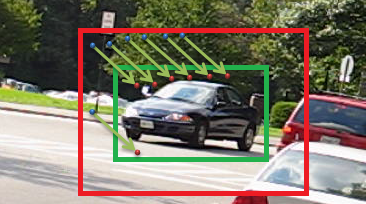
\includegraphics[height=0.285\textheight]{../images/tracking_points.png}
      \caption{Example image of points entering a tracking region (green) due to object motion in a video sequence.}
      \label{figurelabel_entering}
   \end{figure}
\setlength{\belowcaptionskip}{-10pt}

   \begin{figure}[thpb]
      \centering
      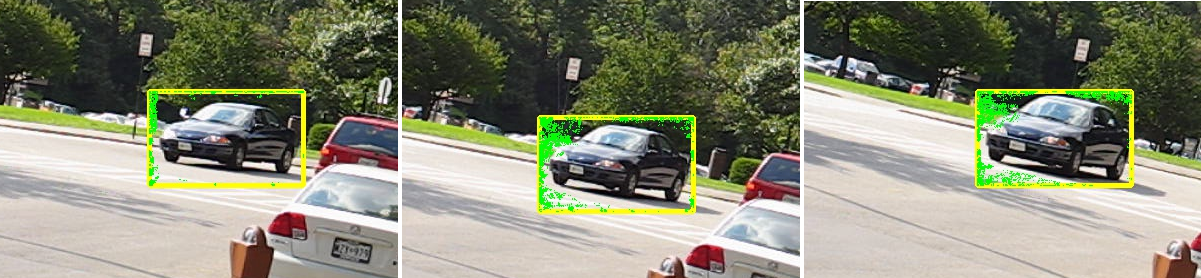
\includegraphics[width=1\textwidth]{../images/pointTr.png}
      \caption{Point tracking using an optical flow method.}
      \label{pointtr}
   \end{figure}


This idea can be applied in several levels in a video sequence. The first method to develop such an algorithm is to do it in the pixel level. The Fig. \ref{pointtr} shows some results by applying 
a dense optical flow technique (Fast Block Matching) in an external window. However, as it can appreciated, the results are rather sparse and after some time, the regularization of the 
optical flow method leads to some of the points being wrongly tracked inside the object boundaries. Both problems, sparsity and tracking errors due to drift and regularization, can be 
overcome by implementing the same idea, but in the superpixel level.
To save computational power, the tracked superpixels are 
limited to the ones that fall inside a control region (red box in the Fig.  \ref{figurelabel_entering}). 

Normally, after several frames, 
the labelled superpixels will almost completely cover the unwanted areas in a dynamic scene. We call this process background segments tracking and the process is summarized in the 
Algorithm \ref{algo1}.  The Fig. \ref{figurelabel_spflow} shows this idea in a real scenario. From left to right, initially the superpixels with 
elements outside the bounding box are labelled as background (green), then, as the sequence changes, the labelled superpixels flow inside the window, giving hints for the model initialization in the background-foreground separation algorithm.

\begin{algorithm}[ht]
\caption{Background regions tracking between a frames A and B}
\label{algo1}
\begin{algorithmic}
\REQUIRE list: $superpixelsA, superpixelsB$, rect: $trackerA, trackerB$, vector: $prev\_labels$

\STATE vector: $new\_labels$
\STATE $computeSuperPixelFlow()$
\FORALL{$superpixel \in superpixelsA$}
    \STATE $matches[superpixel] = getMatchesFromFlow(superpixel)$

	\COMMENT{ Check is previously labelled superpixels fall inside $trackerB$ }
	\IF{$superpixel \in prev\_labels$}
		\STATE $matchAB = superpixelsB[ matches[superpixel] ]$
    		\IF{$matchAB \in trackerB$} 
    			\STATE $new\_labels.push\_back( matchAB )$
    		\ENDIF
	\ENDIF 

	\COMMENT{ Check is new labelled superpixels fall inside $trackerB$ }    
    \IF{$superpixel \notin trackerA$} 
    	    \STATE $matchAB = superpixelsB[ matches[superpixel] ]$
    		\IF{$matchAB \in trackerB$} 
    			\STATE $new\_labels.push\_back( matchAB )$
    		\ENDIF
    	\ENDIF
\ENDFOR

\RETURN $new\_labels$
\end{algorithmic}
\end{algorithm}

At this point, some generic segmentation technique can be connected to the pipeline to refine the segmentation (e.g. region growing). However, graph based segmentation methods are preferred (\cite{c18}\cite{c15}) because the usual user interaction can be replaced by the tracked background regions, and the algorithms are faster and more robust.

   \begin{figure}[thpb]
      \centering
      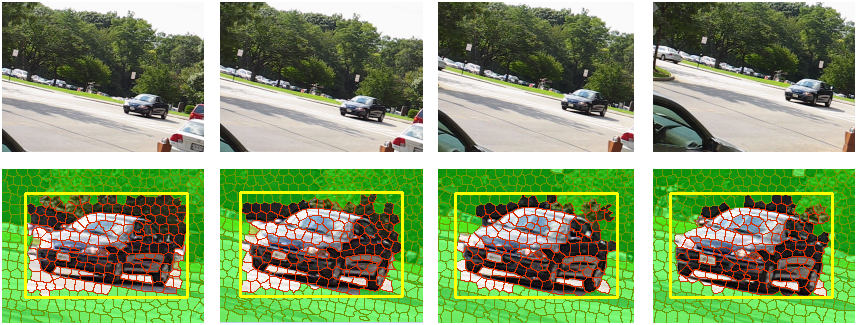
\includegraphics[width=1\textwidth]{../images/suppixflow2.png}
      \caption{Background segments automatic labelling and propagation, the flow goes from left to right.}
      \label{figurelabel_spflow}
   \end{figure}

\subsection{Segmentation results}

Fig. \ref{figurelabel_walking} shows the results for an image sequence where the interest object is the head of a person.
The head tracker and the superpixel flow provide information for better background-foreground separation. The
background-foreground models are updated as the frames go on, giving more robustness for sequential
propagation of the segmentation. The method is tested in the Walking Couple sequence, by allowing only a small amount of iterations in the
graph based segmentation. Observe how the contour in the man's head is correctly delineated when
another person's head occludes part of it. In this case, the superpixels that belong to the woman’s face
were correctly propagated and thus, labelled as background. Its also impressive that the segmentation process recovers after a heavy occlusion.
In this case, the fact that the tracker is also robust to the occlusion is a key factor that help the system maintain a correct segmentation through such a difficult 
case.

   \begin{figure}[thpb]
      \centering
      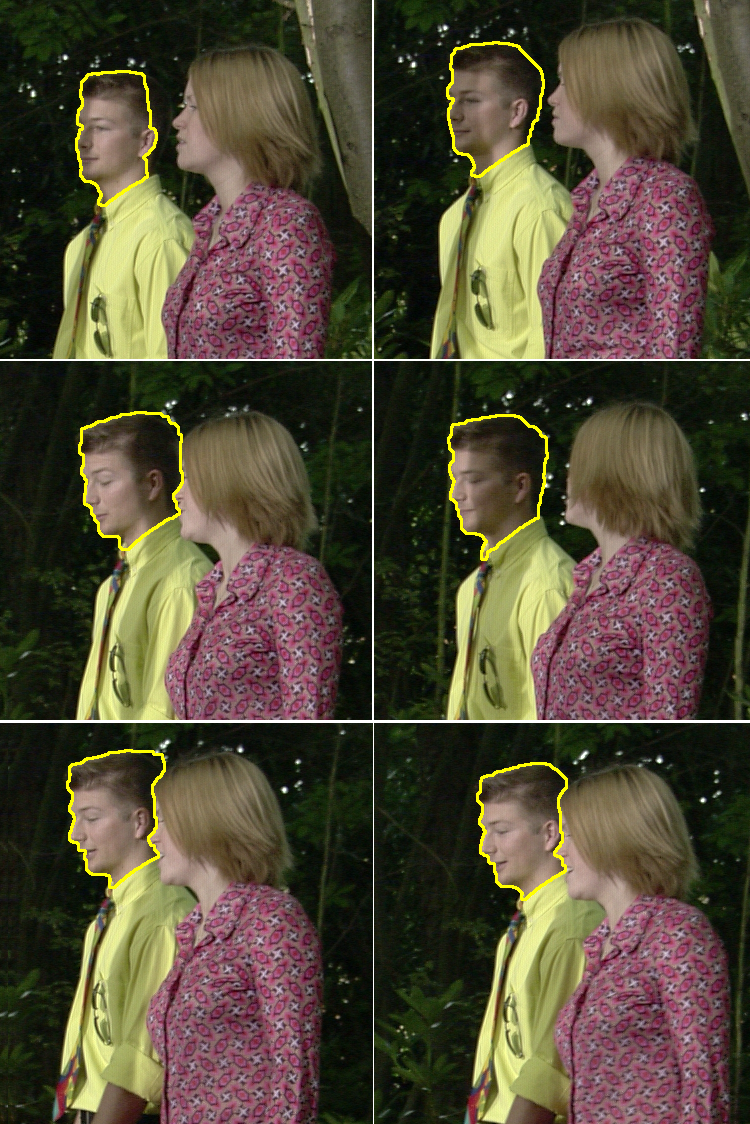
\includegraphics[width=1.0\textwidth]{../images/Sequence.png}
      \caption{Segmentation through the sequence “Walking
	       Couple” (Yellow contour) initialized in the man’s head. The yellow box correspond to the tracker output.
	        The labelled background superpixel are not shown for clarity.}
      \label{figurelabel_walking}
   \end{figure}

In order to understand the effect of including superpixel propagation in a video sequence for object
segmentation, some results are shown in the Fig. \ref{figurelabel_comp}. For these experiments only one iteration is
allowed in the graph-cut based methods. The top row frames (Fig. \ref{figurelabel_comp}) were initialized only with the tracker, 
and the bottom row was initialized with the superpixel tracking technique. 
Observe that in general, the contour delineated is usually better in terms of precision and
stability for the later one. Complete segmentation results can be observed in the Appendix \ref{app:seg}.

   \begin{figure}[thp]
      \centering
      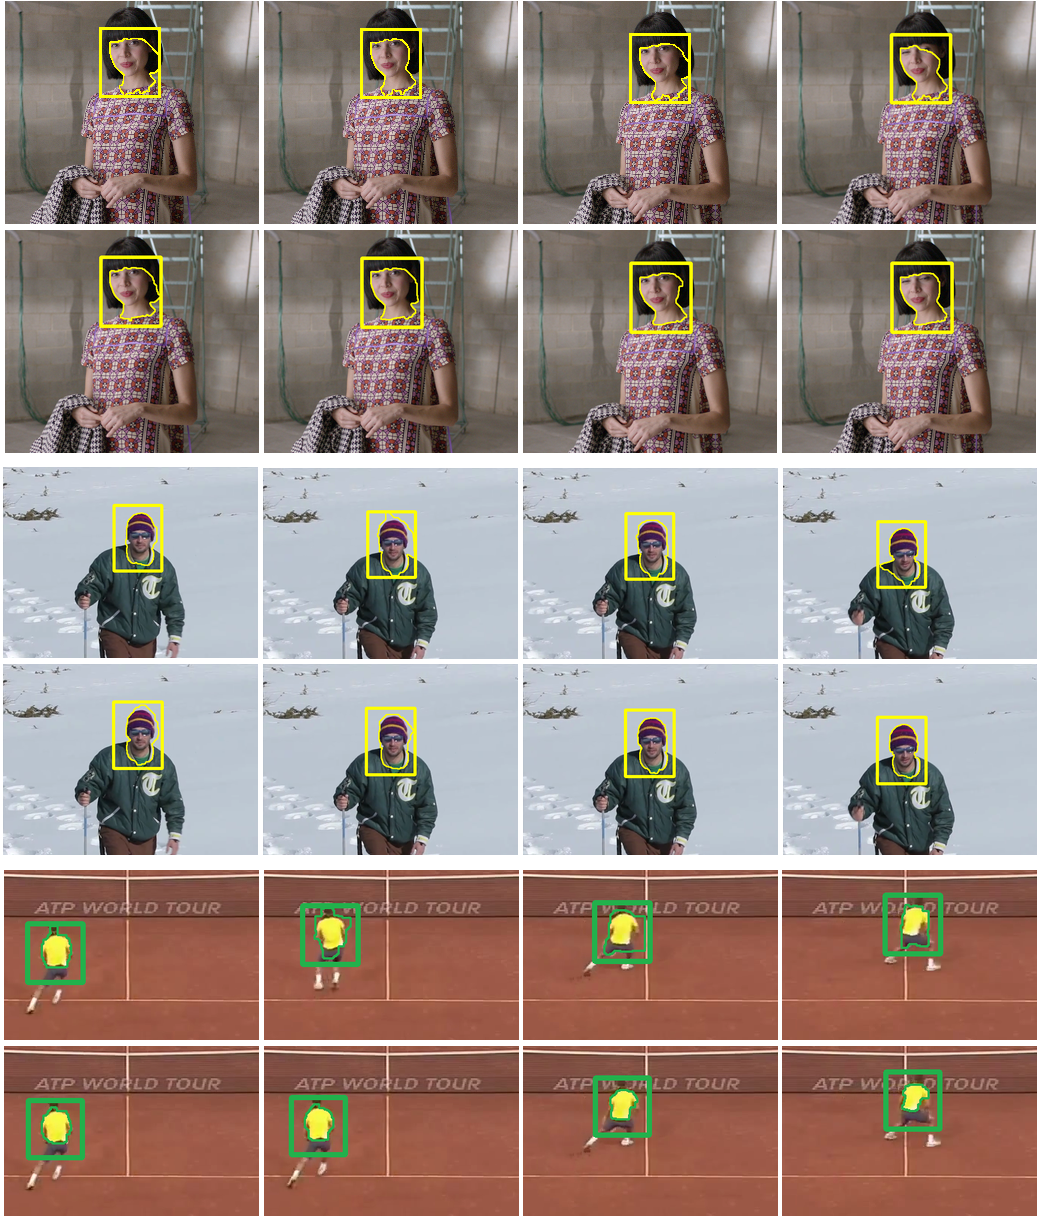
\includegraphics[width=1.0\textwidth]{../images/compareSegm.png}
      \caption{Face segmentation in the “Amelie Retro” and the
	      “Snow shoes” sequences in several different frames, and T-shirt extraction from Tennis sequence. For each
	       group, the Top Row: One-iteration window-based graph-cuts;
	       and the Bottom Row: One-iteration graph-cuts initialized with superpixel tracking.}
      \label{figurelabel_comp}
   \end{figure}
